\documentclass[
  10pt,
  a4paper,
  twocolumn,
]{article}

\usepackage{minted}
\usemintedstyle{bw}
\usepackage{caption}

\usepackage{tikz}
\usetikzlibrary{
  arrows.meta,
  positioning
}
\tikzset{
  every node/.style={draw, align=center, rounded corners},
  -{Stealth[scale=1.2]},
}

\usepackage[cm]{fullpage}

\usepackage{mathpazo} % palatino rm and math
\usepackage[scaled]{helvet} % sf
\usepackage{sourcecodepro} % tt

\usepackage{graphicx}
\usepackage{hyperref}

\usepackage[
	backend=biber
]{biblatex}
\bibliography{references}

\def\mytitle{Puddle: An Operating System for Reliable, High-Level Programming of Microfluidic Devices}
\def\myauthors{Max Willsey, Luis Ceze, and the MISL group}

\def\puddleurl{http://misl.cs.washington.edu/projects/puddle.html}

\hypersetup{
  pdftitle = {\mytitle},
  pdfauthor = {\myauthors}
}

\title{\mytitle}
\author{\myauthors
\\ \small Paul G. Allen School for Computer Science and Engineering
\\ \small University of Washington}
\date{}

\begin{document}

\maketitle

Lab automation technology automatically manipulates small chemical or biological samples to save time and reagents.
While promising, these lab-on-a-chip devices are error-prone and difficult to program.
We propose a runtime system that automates error handling and resource management to provide a system-call-ish interface.
Abstracting away low-level details will make it possible to write high-level programs to automate a variety of lab protocols.

Our talk will begin by presenting the broad applications of lab automation technology.
We will describe the hardware and the challenges of programming it with existing techniques.
We will present our prototype system, explaining how it provides a higher-level programming model.
Finally, we will touch on some future work that these abstractions will enable, including connections to type systems and verification, approximate computing, and molecular computing systems.

\begin{figure}[h]
  \begin{minipage}{0.4\linewidth}
    \footnotesize
    \centering
    \includegraphics[width=0.9\linewidth]{droplet.png}
  \end{minipage}
  \hfill
  \begin{minipage}{0.53\linewidth}
    \begin{minted}[escapeinside=||]{python}
l3 = |\textbf{mix}|(l1, l2)
while get_pH(l3) > 7:
    |\textbf{mix}|(l3)
    acidify(l3)
    ...
# l4 = mix(l1, l3)
# error!
    \end{minted}
  \end{minipage}
  \captionof{figure}{Our prototype DMF chip with droplet tracking.}
  \label{fig:board}
  \vspace{-1em}
  \captionof{figure}{
    A simple program in the Puddle framework.
    The commented-out line would fail because {\tt l1} has already been consumed.
  }
  \label{fig:code}
  \vspace{-2em}
\end{figure}

\section*{Why Microfluidics?}

Microfluidic technology focuses on automatically manipulating small quantities of fluids.
Laboratories typically use these devices to automate experiments, sample preparation, or other processes.

A more advanced programming platform for microfluidics would have applications far beyond just lab automation in chemistry and biology.
If we could reason about programs that manipulate fluids, we could use techniques from programming languages to write safer medical diagnostics.
If writing these programs involved less tedium and was more reliable, lab-based courses could take a more interactive and exploratory approach to education.

In the Molecular Information Systems Group at UW, we are excited about using microfluidic technology to build hybrid molecular-electronic systems.
DNA provides a powerful foundation for data storage \cite{bornholt2016} and computation.
But before we can build practical computer systems that harness the power of molecules, we need a way to automate the liquid handling steps that these protocols entail.
Furthermore, we need an integrated solution that can combine liquid handling with general purpose computation to control the molecular components and analyze data.

\section*{Droplet-based Microfluidics}

While there are several kinds of lab automation devices,
droplet-based microfluidic (DMF) technology is especially promising because of its flexibility.
DMF devices manipulate individual droplets of liquids on a grid of electrodes (\autoref{fig:board}).
Activating electrodes in certain patterns can move, mix, or split droplets anywhere on the chip.

Other microfluidic technologies rely on a fixed network of channels, but DMF
devices are more flexible: think of fixed-function ASICs compared to a CPU.
Unfortunately, the tooling surrounding DMF technology offers little programming abstraction,
and the hardware itself suffers from high failure rates \cite{dmf-review}.

The ``assembly language'' that controls DMF devices is little more than controlling individual electrodes.
For example, the commands to move a droplet from cell (1,3) to cell (2,5) would just be activating the electrodes connecting those cells in sequence.
The program explicitly refers to locations on the chip, and there's no notion of the identity, properties, or even the existence of the droplets!

\begin{figure}
  \hfill
  \begin{minipage}{0.5\linewidth}
    \begin{minted}[fontsize=\small, escapeinside=||]{python}
a = |\textbf{input}|(substance_A)
b = |\textbf{input}|(substance_B)
ab = |\textbf{mix}|(a, b)

|\textbf{heat}|(ab)
    \end{minted}
  \end{minipage}
  \hfill
  \begin{minipage}{0.35\linewidth}
    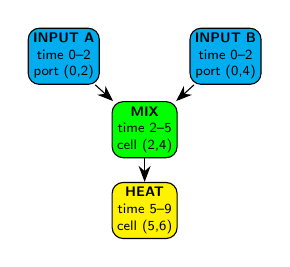
\begin{tikzpicture}
      \tiny \sf
      \node[draw=none] (mid) {};
      \node (A) [left = 5mm of mid, fill=cyan] {
        \textbf{INPUT A} \\
        time 0--2 \\
        port (0,2)
      };
      \node (B) [right = 5mm of mid, fill=cyan] {
        \textbf{INPUT B} \\
        time 0--2 \\
        port (0,4)
      };
      \node (mix) [below = 5mm of mid, fill=green] {
        \textbf{MIX} \\
        time 2--5 \\
        cell (2,4)
      };
      \node (heat) [below = 3mm of mix, fill=yellow] {
        \textbf{HEAT} \\
        time 5--9 \\
        cell (5,6)
      };

      \draw (A) -- (mix);
      \draw (B) -- (mix);
      \draw (mix) -- (heat);
    \end{tikzpicture}
  \end{minipage}
  \hfill

  \caption{
    Fluidic program and the corresponding DAG where the operations have been
    scheduled and placed.
  }
\label{fig:dag}
\end{figure}

Existing work uses place-and-route techniques from VLSI to abstract away specific locations.
In this approach, the program is a DAG that encodes the dependencies of the operations.
\autoref{fig:dag} shows a pseudo-code snippet along with the corresponding DAG.
Tools can take such a DAG and automatically determine when and where to execute each operation \cite{grissom2015open}.
The tool then plans routes for every droplet so that they don't collide on the way.
Importantly, this is all done \emph{ahead of time}.
We don't have to waste computation at runtime creating an execution plan.
Also, we can statically determine if executing a given program on a given chip is possible.

On the other hand, static place-and-route techniques cannot offer error correction or data-dependent control flow.
For example, if the hardware fails when the controller attempts to move a droplet, a static execution plan will just continue, and the plan's model of chip will fall out-of-sync with reality.
If a program branches on the value of a sensor reading, static execution planning gets more complicated.
Simple conditionals can be handled by ``compiling'' basic blocks, but loops and procedures are still out of reach, as there's no ``stack'' on which to dynamically allocation droplets that might be created.

\section*{An Operating System for Fluidics}

With the \href{\puddleurl}{Puddle}\footnote{\tt \puddleurl} framework, we take a dynamic approach to abstracting away the details of DMF programming.
Instead of operating on programs in a restricted language (without functions, loops, or other features),
we instead provide a syscall-like interface that can be used from any programming environment.

\autoref{fig:flow} shows a stack diagram of our system. At the top, the \textsf{API Layer} shows the system calls accessible to the user.
The program deals with opaque handles to droplets (think file descriptors), so the system calls in the \textsf{Control} box \emph{do not have any observable effects to the user}.
In regular operating systems, the only way to observe effects from the \texttt{write} syscall is with other syscalls like \texttt{read};
therefore, the OS doesn't need to execute the \texttt{write} immediately.
Likewise in the Puddle system, we build up a DAG of pending operations.
When the user makes a sensor reading, we are forced to execute those pending operations, take the reading, and return it to the user.

\begin{figure}
  \centering
  \includegraphics[height=0.2\textheight]{information-flow.pdf}
  \caption{Information flow of the Puddle system.}
  \label{fig:flow}
\end{figure}

The core of the Puddle system is placement and routing, shown in the \textsf{Routing} box.
Because all the complications of a programming language (loops, function calls, conditionals) are handled at the user level, the DAG is quite simple.
The DAG knows nothing about control flow; it just records the dependencies of the syscalls the user has made on various handles.
We can use all the same place-and-route algorithms developed by existing work without giving up the ability to write rich programs.

The other major benefit of the dynamic approach is error correction.
The Puddle system can call place and route at runtime, so we can detect and make corrections when droplets do not move properly.
Because users deal only with opaque handles, they cannot inspect the location of a droplet, so error correction is \emph{completely transparent} to the user.
We use a computer vision system to detect the locations of the droplets (shown in \autoref{fig:board}), and we report that information back into the \textsf{Safe Control} component of Puddle that performs error correction.

Finally, the operating system approach allows portability across different microfluidic devices.
As long as the hardware can implement what's in the \textsf{Architecture} box, the Puddle system can provide a high-level programming interface.

\section*{Future Work}

By building an operating system for fluidics instead of a custom, restricted programming language, we gain the ability to do transparent error correction, and we get all the general purpose programming languages.
Importantly, this means that users can now mix regular computation and fluidic manipulation: the same program can run an experiment on the device, analyze the data, and take action based on the results.

\paragraph{Program Analysis}
With our dynamic approach, we lose the ability to statically determine if we can execute a given program on some hardware without running out of space.
This (and all reasoning about the program) gets more challenging since a general purpose language is making the system calls.
However, we hope to apply techniques from programming languages to recover this static reasoning \cite{obt18}.

\paragraph{Approximate Computing}
Many of the operations on a DMF device are low-precision: a \texttt{split} operation may yield two droplets of unequal size.
The error correction system can deal with this to some extent by retrying, but ultimately some level of precision loss will have to be dealt with at the program level.

\paragraph{Molecular Systems}
The Puddle system makes it possible to combine computation with fluidic manipulation.
On top of this, we want to build a library for manipulating and processing synthetic DNA.
Domain-specific abstractions will make it easier to build and reason about hybrid molecular-electronic systems.




% So, a fluidic program in our framework is just a Python program that uses our API.
% fluidic ``syscalls'' like \texttt{mix}, \texttt{input}, \texttt{heat}, etc\.
% call into the runtime system.

% This approach gives both the programmer and us as runtime implementers more flexibility.

% \autoref{fig:code} shows a snippet of a fluidic program written using Puddle.
% The advantages of the API level

\vfill

\renewcommand*{\bibfont}{\tiny}
\printbibliography[heading=none]

\end{document}